\documentclass[mla7]{mla}

\title{How Narrative Works in Outer Wilds}
\author{Dan He}
\professor{Sarah Schoemann}
\course{Game Studies I}
\date{\mladate}
\addbibresource{reference.bib}
\begin{document}
\section{Abstract}
This article briefly reviewed how curiosity works for animals and their
relationship to exploration. Then we have a closer look at how the
curiosity-driven exploration works in the 2019 indie hit \textit{Outer Wilds},
and how it's powering the narrative and integrate it into its gameplay.

\section{Introduction}
\textit{Outer Wilds} is a first-person action-adventure game developed by Mobius
Digital Games and published by Annapurna Interactive in May 2019. The game
features an unnamed alien astronaut as the player character exploring a small
solar system that is stuck in a 22-minute time loop. \textit{Outer Wilds} start
as \cite{beachum2013outer}'s 2013 MFA thesis, and the game won IGF ``Seumas
McNally Grand Prize'' and ``Excellence in Design'' is 2015. They later spent 4
years to form a team and make the game more polished.

\section{Curiosity and Exploration}
\cite{berlyne1966curiosity} said in his \textit{Curiosity and Exploration},
``higher animals spend a substantial portion of their time and energy on
activities to which terms like curiosity and play seem applicable.'' Game
studies scholars are pretty familiar with the idea of play as an activity that
wastes energy, but this also applies to curiosity.

There is a whole page on \cite{nasa}'s website, explaining why human beings
would like to explore. It says ``humans are driven to explore the unknown,
discover new worlds, push the boundaries of our scientific and technical limits,
and then push further.'' Curiosity is closely related to exploration. Even
though people usually explore for different kinds of reasons, as Clint Hocking
mentioned in his 2007 GDC interview by \cite{ruberg2007clint}, he said ``some of
them were motivated by money, some by patriotism or nationalism, some of them by
more of a pure desire to go where people hadn't been'', but we would say that
the strongest and the purest motivation of exploration is curiosity.

To further discuss curiosity-driven exploration, we need first define these two
terms:
\begin{itemize}
\item \textbf{Curiosity} is defined as a need, thirst, or desire for knowledge.
\item \textbf{Exploration} refers to all activities concerned with gathering
  information about the environment.
\end{itemize}
Thus, we could explain curiosity-driven exploration as someone exploring the
environment around with the primary objective of expanding its knowledge of the
surrounding world.

\section{Telling Stories of Distant Places}
One interesting technique used in \textit{Outer Wilds} is by telling stories of
distant places. In \textit{Legend of Zelda: Breath of the Wild}, players start
the game with 12 photos of Hyrule on Link's tablet. One of the main quests in
this game is to find out all the places shot in these photos. Players could
check these photos at any time when they are on their journey. These photos
arouse players' curiosity. They give players some vague information about a
distant place. Players know the existence of the place and they know some
specific details about it, but they don't have any more concrete knowledge of
it. Link could retrieve memory pieces in these 12 spots, so there is some kind
of rewards for players who would like to explore.

In many modern open-world games, the overworld map is only used to navigate
players from place to place. Even though they provide players a huge world, they
are not encouraging players to explore it. Thus, telling stories of distant
places is a way to make players actively participate in the game, comparing to
cut-scene representation or doing repetitive quests.

\section{Narrative in Outer Wilds}
Although the long debate between ludology and narratology had ended for over 15
years, the game industry is still exploring the way to integrate the two parts
naturally. In 2009, \cite{hocking2009ludonarrative} pointed out the
ludonarrative dissonance problem in Bioshock, and this is still something a
majority of the video games are suffering from. Even in 2020, open-world games
like Ghost of Tsushima is still using cinematic cut scenes to tell stories. This
doesn't mean it's not a proper way to implement the narrative, but according
to \cite{frasca2003simulation}'s definition, this is just using the
representation from cinematic media, not simulation.

In \textit{Outer Wilds}, they push this idea further. The player character was
born in a village on a planet called Timber Hearth. After players finished the
tutorial part and can pilot the spaceship, they are allowed to freely explore
the whole solar system. The game provided players with several options at the
end of the tutorial part, but they never told the player where they ``need'' to
go, and what is the goal of the game. The major gameplay of the game is to
explore the universe, reading messages left by another ancient alien species,
which are considered died out many years ago. Players would face unknown natural
phenomenons and constructs built by Nomai, the ancient alien species.

\textit{Outer Wilds} has two kinds of places: one is called ``Curiosities'' and
the other is ``Points-of-Interest''. In the game, ``Points-of-interest'' are
places that are telling the existence of the ``Curiosities'' or other
POIs. Usually, POIs provides enough information for players to investigate on
their own, so that players would never be stuck at a point. There is always
something waiting for them to explore. And there are only 5 ``Curiosities'' in
the game, but each of them is holding the answer to a major narrative
question. All the POIs and Curiosities together consist of a huge ``Web of
Curiosities''. A interesting thing is, these curiosities are not guarded with a
hard lock, which means that you have to complete some quests so that you could
have access to these places. They are only guarded with players' knowledge of
the solar system. Usually, players wouldn't be able to enter these Curiosities
if they haven't gained related knowledge.

\begin{figure}[h]
\centering
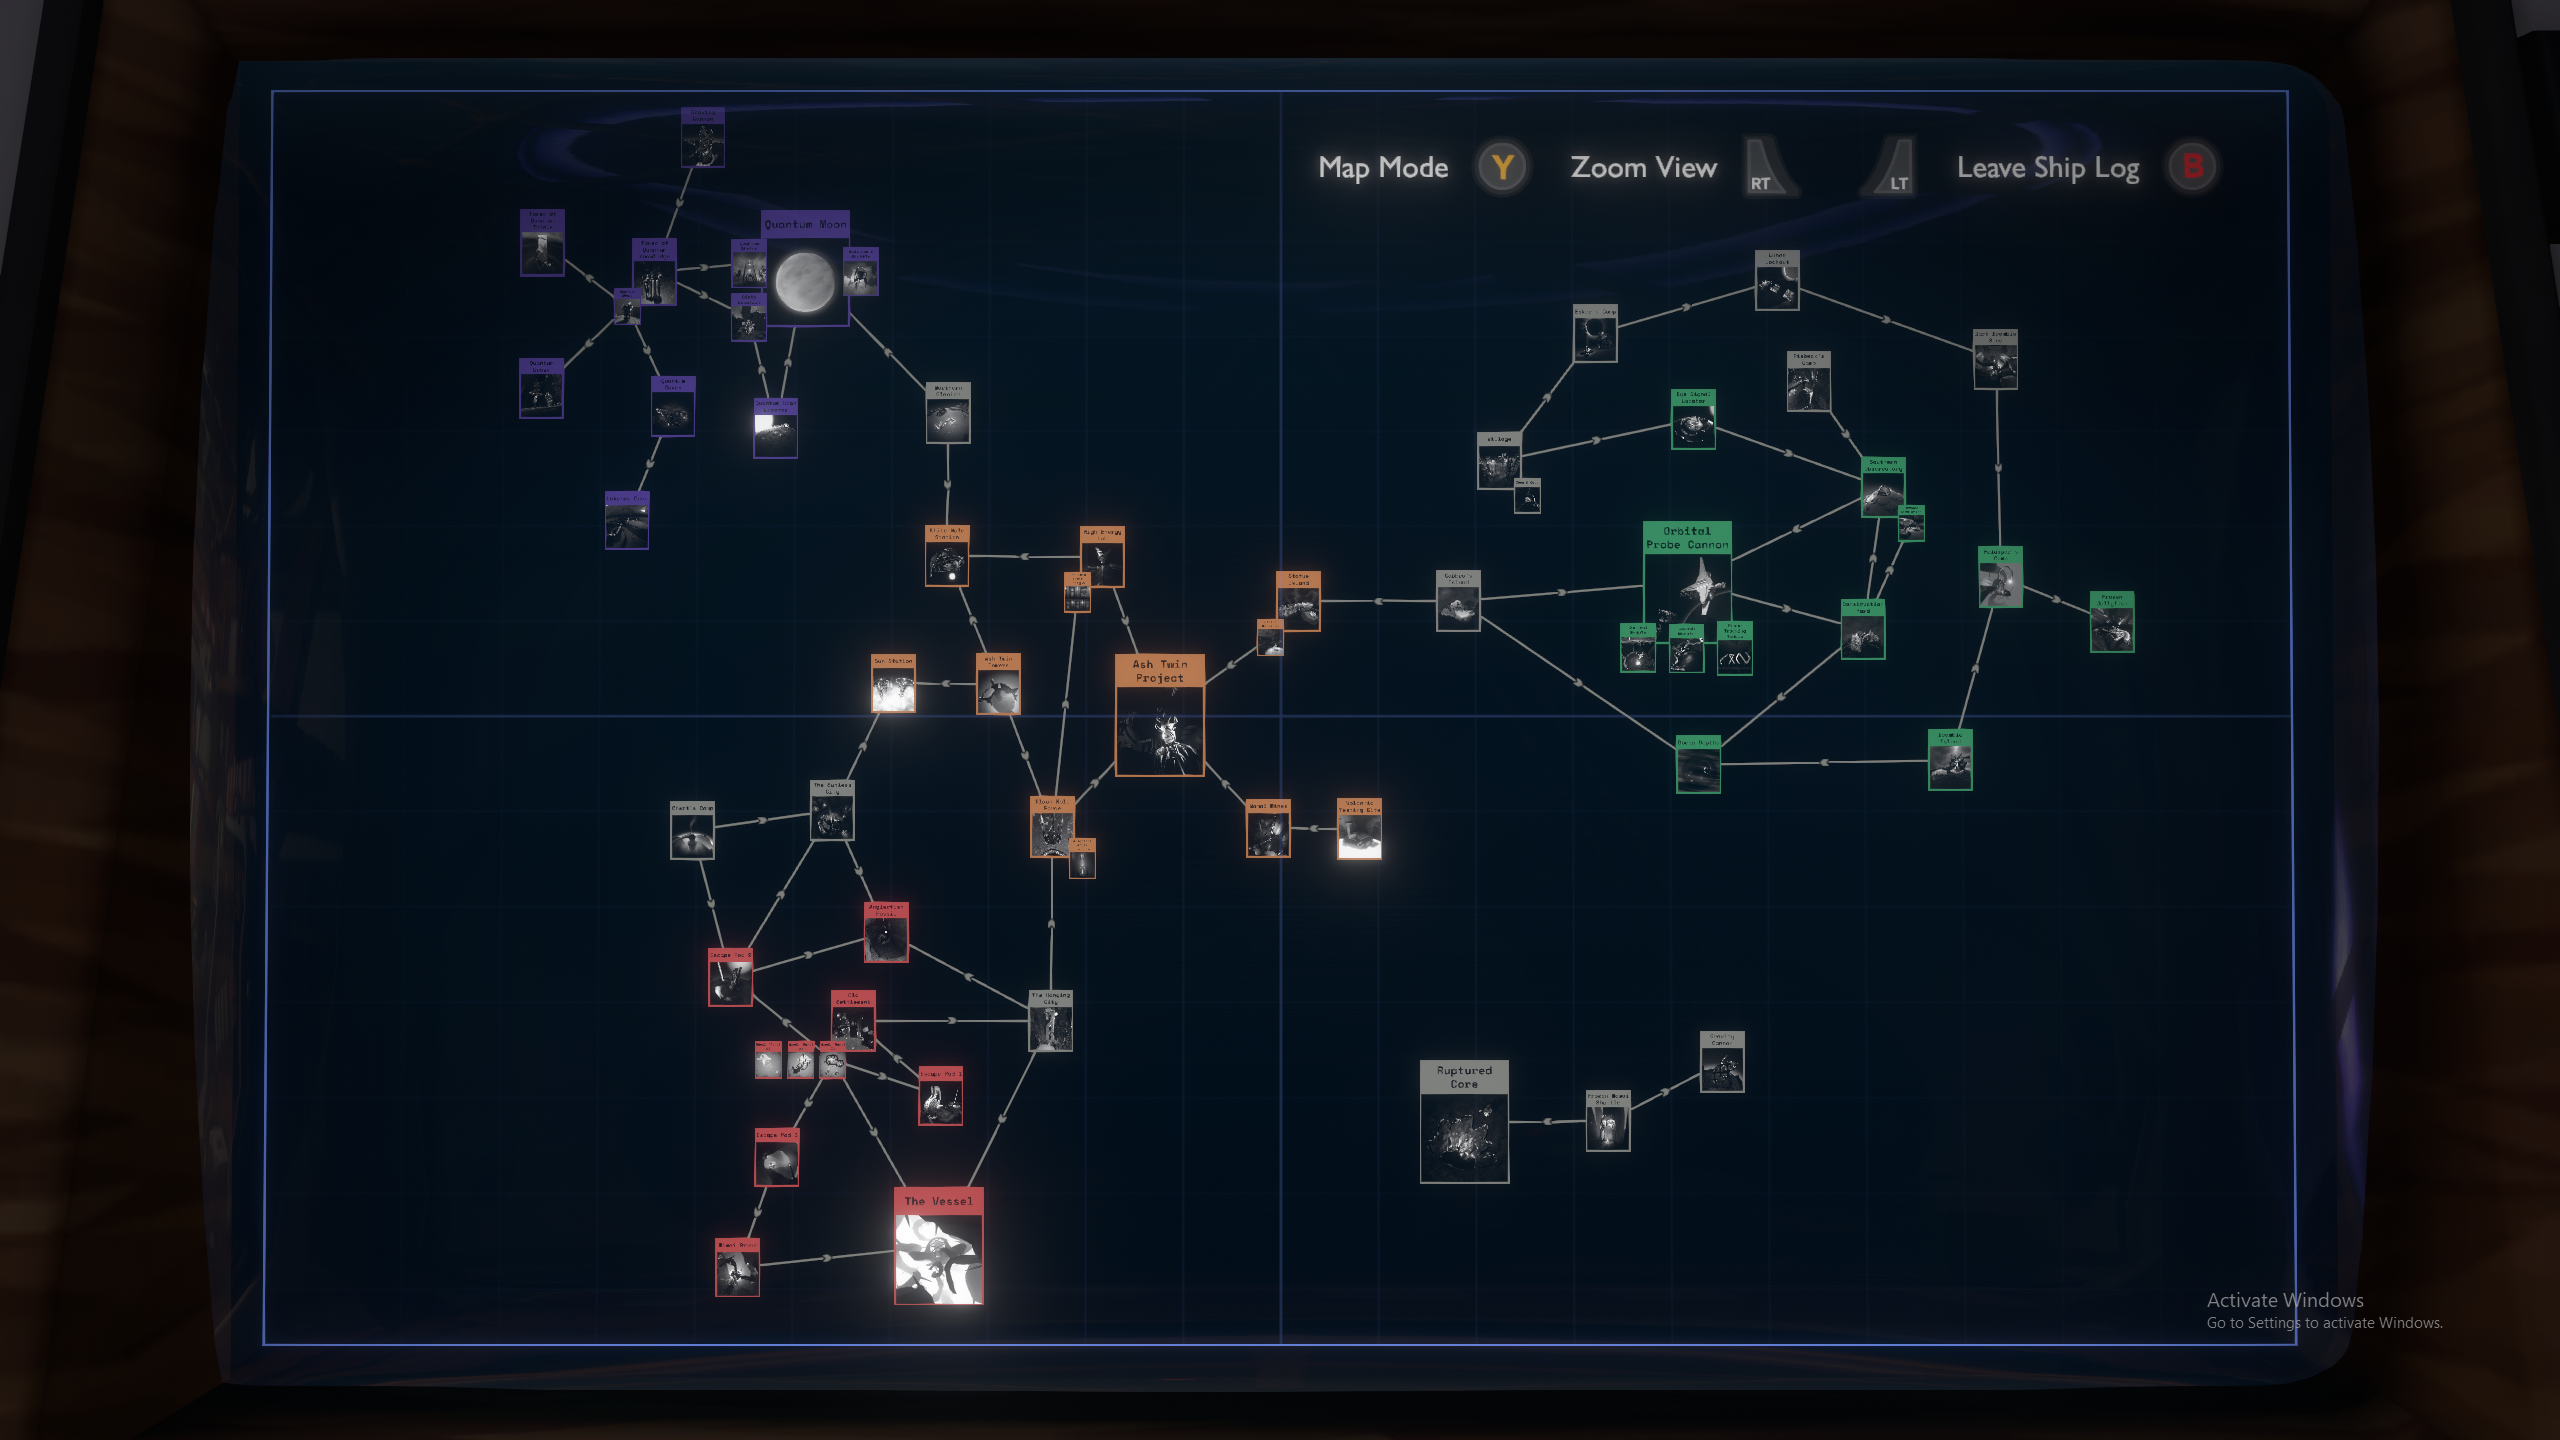
\includegraphics[width=0.7\textwidth]{shiplog}
\caption{Outer Wilds full shiplog}
\end{figure}

By using this ``Web of Curiosities'', \textit{Outer Wilds} naturally embed all
the narrative into its gameplay. The stories are the rewards of players'
exploration, and these stories are pointing to other places that are waiting for
players to explore. This is the embedded narrative mentioned in
\cite{jenkins2004game}' Game Design as Narrative Structure. In the book,
Jenkins argues that detective stories are embedded narrative because ``they
motivate the player's active examination of clues and exploration of spaces and
provide a rationale for our efforts to reconstruct the narrative of past
events.'' Although usually in these open-world games, designers have weaker
control over the narrative structure, this ``Web of Curiosities'' indeed
organized everything into a whole.

Players will gradually learn where the game ends while they explore the solar
system. As we mentioned before, each of the Curiosities is a major part of the
narrative. After players get a full knowledge of the history of Nomai and the
solar system, they would know where to go.

To conclude, the whole process is like, players explore the solar system and
they encounter some POIs; the POIs tell the existence of some Curiosities;
players travel to several POIs to gain full knowledge of the access method to a
specific Curiosity; players visit the curiosity and gain new knowledge of the
narrative part, either the history of Nomai or the solar system or an
explanation to a natural phenomenon; this newly gained story is also a part of
players knowledge of the solar system, which could guide their further
exploration as well. And the Web of Curiosities make sure players won't be
stuck or get lost as each of these elements are connected, which means they are
always pointing to another one.

This curiosity-driven exploration integrates the narrative into the gameplay
itself, and the narrative is also helping players to explore this virtual space
on the mechanic level. Unlike cinematic storytelling, the narrative method in
\textit{Outer Wilds} never breaks the magic circle. All the narrative in this
game are either conversation with other astronauts or reading written messages
left by Nomai. Both of them happen in the fictional world and are not pushing
you away from the controller like what cut scenes do.
\section{Conclusion}
The narrative in \textit{Outer Wilds} could only work in video
games. \cite{juul2001games} once argues in ``Games Telling Stories'' that
``There is an inherent conflict between the \textit{now} of the interaction and
the \textit{past} or 'prior' of the narrative''. But exploring the story of what
has happened to the virtual space skillfully solved this problem. Games like
\textit{Return of the Obra Dinn} also uses this kind of narrative
structure. Video games nowadays are trying to focus more on emergent narrative,
as this could provide endless stories which could make player experience more
diverse, but \textit{Outer Wilds}'s curiosity-driven exploration designed around
the Web of Curiosities successfully integrate the embed narrative into the
gameplay, makes the narrative part and the ludology part feel more like a
whole. The ludonarrative resonance is like the holy grail of game design, and
there are still so many spaces for us to explore.
\begin{paper}
\end{paper}
\begin{workscited}
\printbibliography[heading=none]
\end{workscited}
\end{document}
